\begin{figure}[ht]
  \centering
    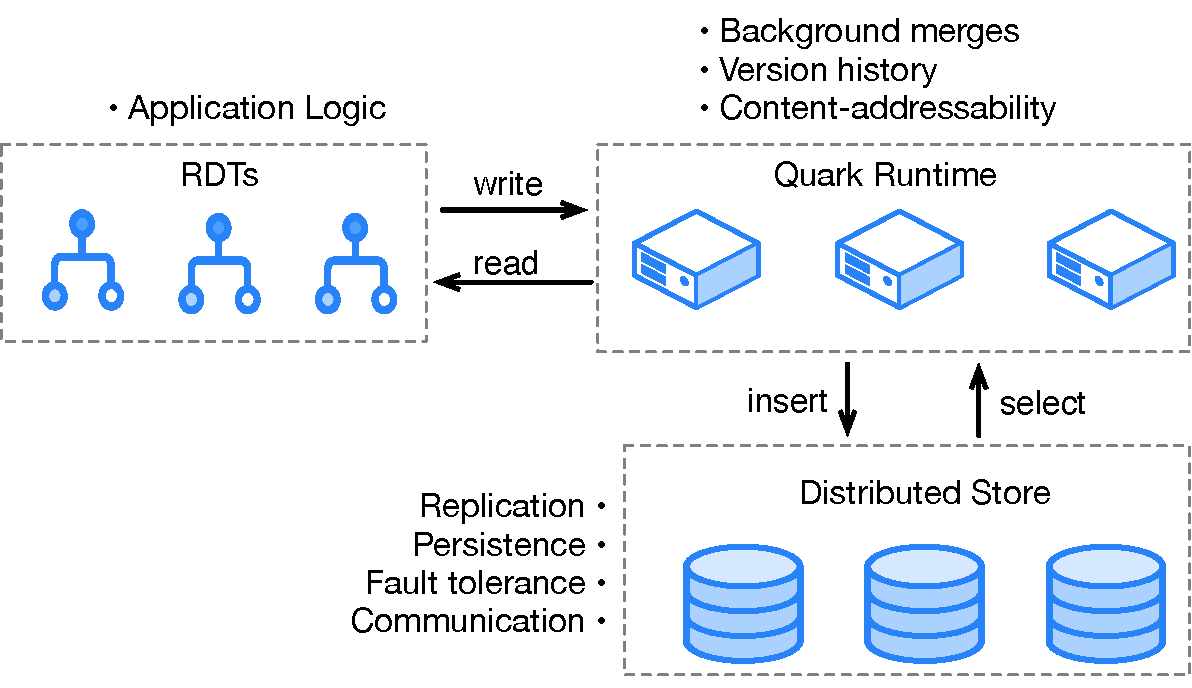
\includegraphics[scale=0.35]{Figures/implementation2}
\caption{\quark implementation architecture}
\label{fig:implementation}
  \vspace*{-0.2in}
\end{figure}

\section{Implementation}
\label{sec:implementation}

We realize a prototype of \quark runtime for MRDTs as a lightweight
shim layer on top of Scylla -- an off-the-shelf distributed data
store~\cite{scylla}. We rely on Scylla for inter-replica
communication, data replication, persistence, and fault tolerance.
\quark translates the high-level MRDT implementations in OCaml to
their low-level representations in the backing store and orchestrates
their well-formed distributed executions.
Fig.~\ref{fig:implementation} illustrates the overall architecture.

The implementation of \quark is a straightforward realization of the
\quark distributed machine described in Sec.~\ref{sec:concrete-sem}.
We manifest each component of the state, namely the branch map $B$,
the value map $N$, and the head map $H$, as a column family (i.e., a
table) in Scylla. The synchronization needed to linearize merges is
implemented with help of Scylla's support for conditional updates (CAS
operations) and expiring columns. The total order among merges is
enforced with help of \C{Quorum} reads and writes. Each user process
is assigned its own replica of the MRDT.  Version vectors are realized
as associative lists and stored in Scylla as blobs.

One key difference between the formalization and the implementation is
in the treatment of MRDT values. Formalization assumes values to be
atomic with no sharing in between them. In practice, however, an MRDT
could be a linked data structure such as a binary tree, and two
such values could share a significant amount of internal structure.
Consequently, the size of the \emph{diff} between two consecutive
versions of a value could be asymptotically less then the size of the
data structure itself, in which case it unreasonable to transfer the
entire data structure over the network. To facilitate the efficient
computation of diffs between versions of data structures, we implement
a \emph{content-addressable store} as a key-value table in Scylla
where key is simply the SHA256 hash of the value. A linked data
structure is stored as a collection of nodes, where each node links to
the other by referring to its hash. The diff between two consecutive
versions of a data structure would simply manifest as new entries in
the content-addressable store reachable from the root of the new
version. The new entries, being new data, are automatically replicated
by Scylla, thus letting us reconstruct the new version at a remote
location. The root hash of the new version is obtained from the value
map $N$, which now maps version vectors to the \emph{hashes} of
values.
